%==================================================================
% BAB 3 (PROPOSAL) — RANCANGAN PENELITIAN
%
% Berkas ini hanya dipakai oleh proposal.tex. Bab 1 dan Bab 2 dipakai
% bersama dengan naskah Tugas Akhir, sehingga "yang dijanjikan" pada
% proposal sama persis dengan yang kelak dibuktikan pada Tugas Akhir.
%==================================================================

\chapter{RANCANGAN PENELITIAN}

\section{Metodologi Penelitian}
Bab ini menjelaskan rancangan penelitian yang akan dilaksanakan untuk menjawab rumusan masalah pada \cref{rq:design} dan \cref{rq:evaluation}. Rancangan metodologi penelitian ini menggunakan pendekatan kuasi-eksperimental (A/B \textit{Testing Playtesting}) yang dipadukan dengan metode rekayasa perangkat lunak (\textit{prototyping}). Alur penelitian secara keseluruhan ditunjukkan pada \cref{fig:alurproposal}.

\begin{figure}[H]
    \centering
    %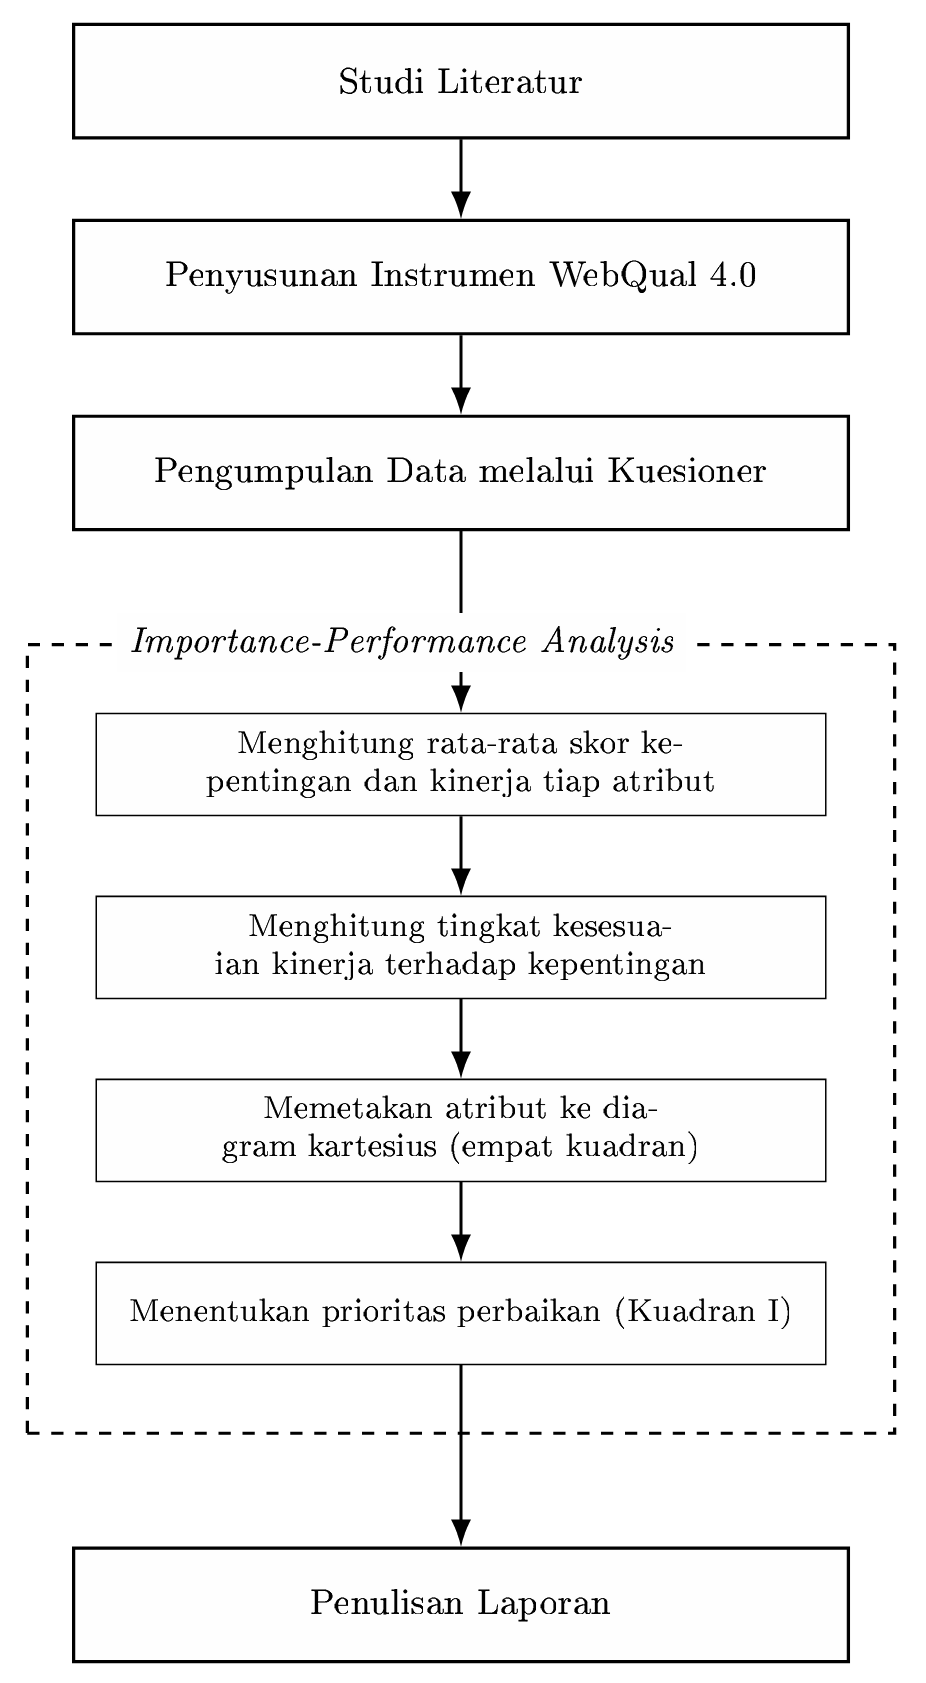
\includegraphics[height=7cm]{metode}   
    \caption{Langkah Penelitian}
    \label{fig:alurproposal}
\end{figure}

\subsection{Studi Literatur}
Pada tahap ini, dilakukan penelaahan mendalam terhadap literatur ilmiah terkini yang mendasari konsep antarmuka diegetik dan penanganan latensi. Literatur utama berfokus pada \textit{Diegetic User Interface} dan kaitannya dengan \textit{Player Immersion} serta \textit{User Experience}, rekayasa \textit{Asynchronous State Machine} pada \textit{game engine} untuk memisahkan eksekusi animasi fisik karakter dari \textit{background thread}, serta pengukuran \textit{Perceived Latency} dan \textit{Player Experience} (PX).

\subsection{Perancangan Prototipe Game 2D dan Skenario A/B Testing}
Pengembangan prototipe dirancang 2D dengan latar berada di Kampus Unika Atma Jaya BSD. Untuk menguji efektivitas penyamaran latensi, dibuat dua skenario perlakuan (\textit{treatment groups}) dengan durasi jeda waktu komputasi AI yang disimulasikan menggunakan fungsi pengacakan waktu (\textit{randomized delay/randint}) pada rentang X detik:
\begin{itemize}
    \item \textbf{Skenario A (\textit{Baseline / Non-Diegetic Group})}: Pemain mengajukan pertanyaan teks, lalu NPC Pustakawan berada dalam kondisi diam (\textit{idle/frozen}). Layar menampilkan komponen \textit{Non-Diegetic} UI berupa \textit{Loading Bar} atau teks "\textit{Thinking...}" selama X detik sebelum jawaban teks NPC muncul.
    \item \textbf{Skenario B (Eksperimen / \textit{Diegetic Latency Masking Group})}: Pemain mengajukan pertanyaan teks, lalu NPC memicu skrip animasi fisik kontekstual secara \textit{asynchronous} (misal: berjalan menuju rak buku atau memeriksa berkas dokumen) selama X detik yang persis sama, lalu NPC kembali ke meja dan jawaban teks muncul.
\end{itemize}

\subsection{Penyusunan Instrumen Evaluasi}
Instrumen penelitian disusun menggunakan kuesioner tertutup berskala Likert lima poin, sebagaimana disajikan pada \cref{tab:likertproposal}. Butir kuesioner dirancang untuk mengukur tiga variabel utama: \textit{Perceived Latency} (mengukur persepsi wajar/tidaknya waktu tunggu), \textit{Player Immersion} (mengukur penjagaan kontinuitas cerita fiksi \textit{game}), dan \textit{Player Retention \& Experience} (mengukur kenyamanan dan keinginan melanjutkan permainan).

\subsection{Populasi dan Sampel}
Populasi target penelitian ini adalah mahasiswa Teknik Aktif Universitas Katolik Atma Jaya BSD. Teknik pengambilan sampel menggunakan \textit{Convenience Sampling} dengan catatan bahwa mereka bersedia mengikuti prosedur \textit{playtesting} dua skenario interaksi secara utuh. Ukuran sampel ditetapkan sebanyak ~30 responden.

\subsection{Pengumpulan Data (Prosedur Playtesting)}
Pengumpulan data dilaksanakan melalui sesi \textit{user playtesting} langsung dengan protokol \textit{Within-Subjects Design} di mana setiap responden mencoba kedua skenario secara bergantian dengan urutan acak (\textit{counterbalancing}) untuk menghindari \textit{order bias}. Setelah menyelesaikan kedua skenario, responden mengisi kuesioner secara mandiri.

\begin{table}[H]
    \centering
    \caption{Skala Likert yang akan digunakan}
    \label{tab:likertproposal}
    \small
    \begin{tabular}{|c|l|}
        \hline
        \textbf{Skor} & \textbf{Pernyataan} \\ \hline
        1 & Sangat Tidak Setuju (STS) \\ \hline
        2 & Tidak Setuju (TS)         \\ \hline
        3 & Netral (N)                \\ \hline
        4 & Setuju (S)                \\ \hline
        5 & Sangat Setuju (SS)        \\ \hline
    \end{tabular}
\end{table}

\subsection{Teknik Analisis Data}
Data yang terkumpul dianalisis melalui dua tahap. Pertama, \textbf{Analisis Deskriptif} untuk menghitung nilai rata-rata (\textit{mean}), standar deviasi, dan median dari skor ketiga variabel utama. Kedua, \textbf{Uji Komparatif Statistik (Uji Beda)} untuk menguji signifikansi perbedaan antara Skenario A dan Skenario B. Uji ini diawali dengan Uji Normalitas (Shapiro-Wilk) dan dilanjutkan dengan \textit{Paired Sample t-Test} (jika normal) atau \textit{Wilcoxon Signed-Rank Test} (jika tidak normal). 
%dengan tingkat signifikansi $\alpha=0,05$.

\subsection{Penulisan Laporan}
Tahap akhir adalah penyusunan laporan yang merangkum seluruh proses dan hasil
penelitian menjadi naskah Tugas Akhir yang utuh.

\section{Matriks Keterkaitan Penelitian}
Agar penelitian tetap terarah, setiap rumusan masalah dipetakan terhadap data dan teknik analisis yang direncanakan, sebagaimana ditunjukkan pada \cref{tab:linkageproposal}.

\begin{table}[H]
    \centering
    \caption{Rencana keterkaitan penelitian}
    \label{tab:linkageproposal}
    \small
    \begin{tabularx}{\linewidth}{|c|X|X|}
        \hline
        \textbf{RQ} & \textbf{Data yang direncanakan} & \textbf{Teknik analisis} \\ \hline
        \cref{rq:design}    & Spesifikasi \textit{Asynchronous State Machine} \& \textit{Asset} animasi 2D NPC & Perancangan Sistem (\textit{Prototypes Engineering}) \\ \hline
        \cref{rq:evaluation} & Skor kuesioner \textit{Perceived Latency}, \textit{Player Immersion}, dan \textit{Player Retention} & Analisis Deskriptif dan Uji Beda Statistik \\ \hline
    \end{tabularx}
\end{table}

\section{Rencana dan Jadwal Penelitian}
Rencana pelaksanaan penelitian disusun selama enam bulan sebagaimana ditunjukkan pada \cref{tab:jadwal}. Sel yang diarsir menandakan bulan pelaksanaan tiap kegiatan.

\definecolor{jadwalisi}{gray}{0.25}
\begin{table}[H]
    \centering
    \caption{Rencana dan jadwal penelitian}
    \label{tab:jadwal}
    \small
    \begin{tabular}{|c|l|*{6}{>{\centering\arraybackslash}p{0.6cm}|}}
        \hline
        \multirow{2}{*}{\textbf{No.}} & \multirow{2}{*}{\textbf{Kegiatan}}
          & \multicolumn{6}{c|}{\textbf{Bulan}} \\ \cline{3-8}
         & & 1 & 2 & 3 & 4 & 5 & 6 \\ \hline
        1. & Studi Literatur \& Penyusunan Instrumen & \cellcolor{jadwalisi} & \cellcolor{jadwalisi} &                       &                       &                       &                       \\ \hline
        2. & Perancangan \& Pembuatan Aset Animasi 2D &                       & \cellcolor{jadwalisi} & \cellcolor{jadwalisi} &                       &                       &                       \\ \hline
        3. & Implementasi Prototipe Skenario A \& B  &                       &                       & \cellcolor{jadwalisi} & \cellcolor{jadwalisi} &                       &                       \\ \hline
        4. & Sesi \textit{Playtesting} \& Pengumpulan Data &                       &                       &                       & \cellcolor{jadwalisi} &                       &                       \\ \hline
        5. & Analisis Data Statistik \& Uji Beda     &                       &                       &                       &                       & \cellcolor{jadwalisi} &                       \\ \hline
        6. & Penyusunan Laporan Akhir \& Sidang TA   &                       &                       &                       &                       & \cellcolor{jadwalisi} & \cellcolor{jadwalisi} \\ \hline
    \end{tabular}
\end{table}